
\documentclass[11pt]{article}

 \renewcommand*\familydefault{\sfdefault}
\usepackage[sort,nocompress]{cite}
\usepackage[small,bf,up]{caption}
\renewcommand{\captionfont}{\footnotesize}
\usepackage[left=1in,right=1in,top=1in,bottom=1in]{geometry}
\usepackage{graphics,epsfig,graphicx,float,subfigure,color}
\usepackage{algorithm,algorithmic}
\usepackage{amsmath,amssymb,amsbsy,amsfonts,amsthm}
\usepackage{url}
\usepackage[sf,bf,tiny]{titlesec}
 \usepackage[plainpages=false, colorlinks=true,
   citecolor=blue, filecolor=blue, linkcolor=blue,
   urlcolor=blue]{hyperref}

\usepackage{listings}
% global settings for listings package
\lstset{
basicstyle=\footnotesize,
stringstyle=\ttfamily,
numbers=left,
numberstyle=\tiny,
stepnumber=1,
numbersep=5pt,
escapeinside={(*}{*)}
}

\newcommand{\todo}[1]{\textcolor{red}{#1}}
% see documentation for titlesec package
% \titleformat{\section}{\large \sffamily \bfseries}
\titlelabel{\thetitle.\,\,\,}

\renewcommand{\baselinestretch}{0.994}
\newcommand{\bs}{\boldsymbol}
\newcommand{\alert}[1]{\textcolor{red}{#1}}

\setlength{\emergencystretch}{20pt}

\begin{document}

\begin{center}
\vspace*{-2cm}
{\small MATH-UA.0252-003 (Georg Stadler, NYU Courant)}
\end{center}
\vspace*{.5cm}
\begin{center}
\large \textbf{%%
Spring 2022: Numerical Analysis}\\
\textbf{ Assignment 1 (due Feb.\ 13, 2022 at 11:59pm ET)}
\end{center}

\noindent\fbox{%
  \parbox{.97\textwidth}{%
    \vspace*{-2ex}
    \paragraph{Homework submission.}
    Homework assignments must be submitted through Gradescope.  Please
    hand in cleanly handwritten or typed (preferably with \LaTeX---I
    provide the source files of these assignments if you want to
    use them to learn \LaTeX) homeworks.  If you are required to hand
    in code or code listings, this will explicitly be stated on that
    homework assignment (if nothing is stated, you are not required to
    hand in code listings).\\[-5ex]
    \paragraph{Collaboration.}
    NYU's integrity policies will be enforced.  You are encouraged to
    discuss the problems with other students in person or  on Campuswire.  However,
    you must write (i.e., type) every line of code yourself and also
    write up your solutions independently. Copying of any portion of
    someone else's solution/code or allowing others to copy your
    solution/code is considered cheating.\\[-5ex]
    \paragraph{Plotting and formatting.}
    Plot figures carefully and think about what you want to illustrate
    with a plot. Choose proper ranges and scales (\texttt{semilogx,
      semilogy, loglog}), always label axes, and give meaningful
    titles. Sometimes, using a table can be useful, but never submit
    pages filled with numbers. Discuss what we can observe in and
    learn from a plot.  Use \texttt{format compact} and other format
    commands to control outputs.  When you create figures in MATLAB
    (or Python, Julia), please export them in a vector graphics format
    (.eps, .pdf, .dxf) rather than raster graphics or bitmaps (.jpg,
    .png, .gif, .tif). Vector graphics-based plots avoid pixelation
    and thus look much cleaner. \\[-5ex]
    \paragraph{Programming.}
    This is an essential part of this class. We will use MATLAB for
    demonstration purposes in class, but you are free to use other
    languages (Python, Julia). Basic programming skills are crucial
    for many jobs, so this is also a good chance to get more
    comfortable with it, if you aren't already.  In your programs,
    please use meaningful variable names and try to write clean, concise
    and easy-to-read code. Comments for explanation are a crucial part
    of every program. }%
  \hspace{3ex}
}

% ---------------------------------------------------------------

\begin{enumerate}
% ---------------------------
\item {\bf [1+1+1+1pt]}  Let $f(x) = e^x - x^2 -2x - 1 $ and $g(x) = 2 \ln
  (x+1)$, where $x\in(-1,\infty)$.
\begin{enumerate}
\item Verify that the roots of $f(x)$ are the same as the fixed points
  of $g(x)$.
\item Sketch $y = g(x)$, $y =x$ and indicate all fixed points (sketch
  by hand or plot with a computer). You don't need to calculate
  them. (Hint for the sketch: Note that $g'(0)>1$).
\item Use Brouwer's fixed point theorem to argue the existence of a
  fixed point $\xi$ in the interval $[a,b] = [e-1 , e^2 - 1]$.
\item Use the contraction mapping theorem to show that $\xi$ is the
  only fixed point in the interval $[e-1,e^2 -1]$.
\end{enumerate}


%%%%%%%%%%%%%%%%%%%%%%%%%%%%%%%
\item {\bf [2+2pt]} Stability of fixed points.
\begin{enumerate}
\item For each of the three functions (solid lines) depicted below,
	\begin{enumerate}\setlength{\itemsep}{0.2cm}
		\item[(i)]  Write down the approximate values of the
                  fixed points (as estimated by eye).
		\item[(ii)] State for each fixed point, whether it is
                  stable, unstable or neither of the two.
	\end{enumerate}
	\begin{figure}[h!]
	\centering
	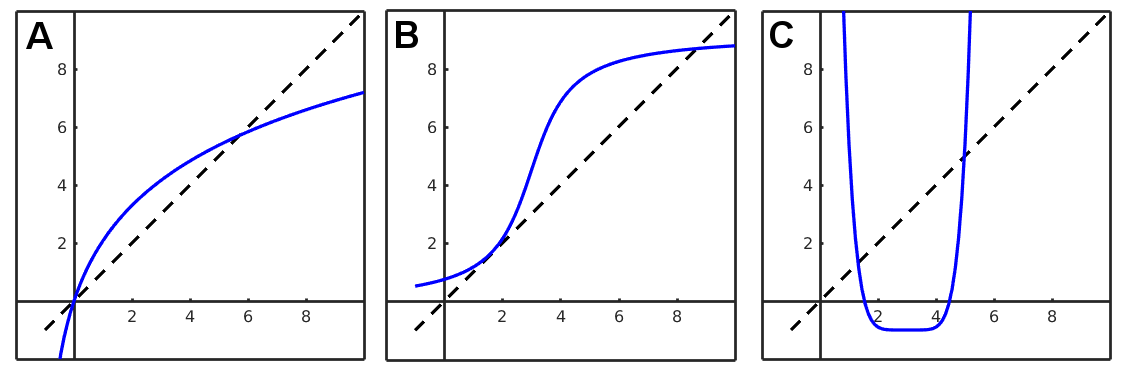
\includegraphics[width=\textwidth]{fig}
	\end{figure}

      \item   You are given the first ten iterates of two sequences, $x_k$ and $y_k$, both of which converge to zero:\\
\begin{center}
\begin{tabular}{|c|c|c|}
\hline
  $k$ & $x_k$ & $y_k$ \\
\hline
0 & 1.0000000000000 & 1.0000000000000 \\
1 & 0.3000000000000 & 0.6648383611734 \\
2 & 0.0900000000000 & 0.4404850619261 \\
3 & 0.0270000000000 & 0.2895527955097\\
4 & 0.0081000000000 & 0.1869046766665\\
5 & 0.0024300000000 & 0.1155100169867\\
6 & 0.0007290000000 & 0.0638472856062\\
7 & 0.0002187000000 & 0.0254178900244\\
8 &0.0000656100000 & 0.0032236709627\\
9 &0.0000196830000 & 0.0000080907744\\
10 &0.0000059049000 & 0.0000000000001\\
\hline
\end{tabular}
\end{center}
\vspace{0.5cm}
\begin{enumerate}
\item[(i)] What is (most likely) the order of convergence of $x_k$?
  Explain your answer.
\item[(ii)]What is (most likely) the order of convergence of $y_k$? Explain your answer\footnote{Note that we typically thing of local
  convergence, i.e., close to the limit point.}.
\end{enumerate}
\end{enumerate}


%%%%%%%%%%%%%%%%%%%%%%%%%%%%%

\item {\bf [2+1+1pt]}  Let $g$ be defined on $[5\pi/8, 11\pi/8]$.
  \[
  g(x)=x+0.8\sin{x}.
  \]
  \begin{enumerate}
  \item Determine the (smallest possible) Lipschitz constant $L$.
%  \item What can
%    you say about the asymptotic rate of convergence?
  \item How many
    iterations are required to increase the accuracy by a factor of
    100, i.e., given some $x_0\in [1,2]$, when what is $k$ such that
    you can guarantee that $|x_k-\xi|\le 10^{-2}|x_0-\xi|$?
  \item Starting with initial guess $x_0=5\pi/8$, compute the first
    fixed point iterate $x_1$ and use it, together with the
    Lipschitz constant you found, to compute after how many fixed point
    iterations $k$ you can be certain that $|\xi-x_k|<10^{-10}$.
  \end{enumerate}

%%%%%%%%%%%%%%%%%%%%%%%%%%%%

% \item {\bf [3pt]} We search for solutions in $[1,2]$ to the equation
%   $$x^3 -3x^2 + 3 = 0.$$
%   \begin{enumerate}
%   \item Compute the first iterates $x_0,\ldots,x_5$ of the secant
%     method in $[1,2]$.
%   \item Compute the first iterates $x_0,\ldots,x_5$ using Newton's
%     method with starting value $x_0=1.5$.
%   \item Compute the first iterates using Newton's method with starting
%     value $x_0=2.1$. Sketch the equation graph and try to explain the
%     behavior.
%   \end{enumerate}

  \item {\bf [1+1+1+1pt]}
  The equation
  $$
  f(x):=x^2 - 5 = 0,
  $$ has a single root $\xi = \sqrt{5} \approx 2.2361 \hdots$ in the
  interval $[1,3]$.  Consider the fixed point iteration $x_{k+1} = g(x_k)$,
  where $g$ is defined as one of the following options:
  \begin{itemize}
  \item $g_1(x) = 5 + x - x^2$,
  \item $g_2(x) = 1+x - \frac{1}{5}x^2$,
  \item $g_3(x) = \frac{1}{2}x + \frac{5}{2x^2}$.
  \end{itemize}
  \begin{enumerate}
    \item Identify the fixed point functions for which the fixed point is also a root of
      $f$.
    \item For the cases where computing the fixed point is equivalent
      with solving $f(x)=0$, discuss whether the fixed point
      iteration is guaranteed to converge in some neighborhood of
      $\xi$.
    \item If the iteration in b) is guaranteed to converge,
      compute the value of
      $$
      \lim_{k\rightarrow\infty}\frac{|x_{k+1} - \xi|}{|x_{k} - \xi|}
      $$
      \emph{Hint:} Everything is easier with the mean value theorem!
    \item Give Newton's method for solving $f(x)=0$ and, for given
      starting value $x_0=2$ compute the first Newton iterate $x_1$.
  \end{enumerate}

%%%%%%%%%%%%%%%%%%%%%%%

\item {\bf [3pt]} 
Define the function $g$ by $g(0) = 0$, $g(x) = -x\sin^2(1/x)$ for $0 < x \leq 1$.  Show that $g$ is continuous, and that $0$ is the only fixed point of $g$ in the interval $[0,1]$.  By considering the iteration $x_{n+1} = g(x_n)$, with $x_0 = 1/(k\pi)$ and $x_0 = 2/((2k+1)\pi)$, where $k$ is an integer, show that using the definition of stability provided in class, $\xi=0 $ is neither stable nor unstable.

%%%%%%%%%%%%%%%%%%%%%%%

\item {\bf [2+2pt]} Raytracing is an algorithm that involves finding the
  point at which a ray (a line with a direction and an origin)
  intersects a curve or surface. We will consider a ray intersecting
  with an ellipse. The general equation for an ellipse is
\[
\left( \frac{x}{a} \right)^{2} + \left( \frac{y}{b} \right)^{2} - 1 = 0
\]
and the equation for a ray starting from the point $P_0 = [x_0,y_0]$
in the direction $\textbf{V}_0 = [u_0,v_0]$, is
\[
\textbf{R}(t) = [x_0 + t u_0,y_0 + t v_0]
\]
where $t \in [0,\infty)$ parameterizes the ray. In this problem we
  will take $a = 3$, $b=2$, $P_0 = [0,b]$, $\textbf{V}_0 =
  [1,-0.3]$. Using your favorite root finding algorithm write a code
  which computes the intersection of the given ray and the ellipse and
  plot your results. .
\begin{enumerate}
	\item Plug the equation for the ray, $\textbf{R}(t)$, into the
          equation for the ellipse and analytically (with pen and
          paper) solve for the value of $t$ which gives the point of
          intersection, call it $t_i$.
	\item Perform the same calculation numerically using your
          favorite root finder. Report your answer to within an error
          of $10^{-6}$ and justify how you found the minimum number of
          iterations required to achieve this tolerance. Also report
          the point of intersection $P_i = \textbf{R}(t_i)$
\end{enumerate} 

\item {\bf [4pt, extra credit]} If the walls of the ellipse are perfect mirrors, a
  ray of light will reflect infinitely around within the ellipse. We
  will write an algorithm to compute it's trajectory. Using the same
  parameters as the previous problem. Implement the following
  algorithm for 50 steps.
	\begin{figure}[h!]
	\centering
	\includegraphics[width=.6\textwidth]{fifty_steps}
	\end{figure}
At step $k$ of the process, we are given a point on the ellipse $P_k =
[x_k,y_k]$ and a ray direction $\textbf{V}_k = [u_k,v_k]$
\begin{enumerate}
	\item Using $P_k$ and $\textbf{V}_k$ and your favorite root
          finder, calculate the value of $t$ corresponding to the
          point of intersection call it $t_i^k$.
	\item Compute $P_{k+1} = \textbf{R}(t_i^k)$.
	\item Compute the normal vector at $P_{k+1} = [x_{k+1},
          y_{k+1}]$ as $\textbf{N}_{k+1} = [\frac{b}{a} x_{k+1},
          \frac{a}{b} y_{k+1}]$. Using this compute the UNIT normal
          $\textbf{n}_{k+1} =
          \textbf{N}_{k+1}/||\textbf{N}_{k+1}||_2$.
	\item Compute the unit ray vector $\textbf{w}_k =
          \textbf{V}_k/||\textbf{V}_k||_2$ and update the new ray
          vector using the reflection formula
	\[
	 \textbf{V}_{k+1} = \textbf{w}_k - 2 \left( \textbf{w}_k \cdot
         \textbf{n}_{k+1}\right) \textbf{n}_{k+1}
	\]
        \item repeat from step 1 using $\textbf{V}_{k+1}$ and $P_{k+1}$.
\end{enumerate} 
 Plot the trajectory (all of the points that you computed with line
 connecting them) as well as the ellipse. Also report the 50th point
 of intersection. Note that the shape that encloses all of the
 reflected rays is called a 'caustic'.



\end{enumerate}

\end{document}
